\scanpage{14}
\mspage{12}

grable''. \inserted{[}Enfin, lorsque S donc $X_K$ est géométriquement connexe, et que K peut se plonger dans le corps des complexes $\underline C$, alors la notion de module cohérent à \unsure{conn|comn}\inserted{ex}ion intégrable sur $X_K$ s'interprète en termes de représentations linéaires \inserted{(complexes)} du groupe fondamental \deleted{\unsure{du|de}} transcendant de $X_{\underline C}^{\mathrm{an}}$, de façon bien connue. Si par exemple le groupe fondamental transcendant est le groupe unité, alors on conclut par descente que tout Module cohérent stratifié sur $X_K$ est trivial, ce qui en termes de S s'énonce en disant que tout cristal de modules cohérents sur S est isogène à un cristal ``con\unsure{st|ss}ant'', i.e. \deleted{image} \inserted{à un cristal} qui est l'image inverse d'un cristal sur k, (lui-même défini par un module de type fini sur W). De ceci et de la rigidité de la notion de cristal on déduit\figure{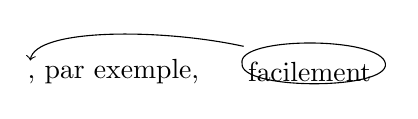
\begin{tikzpicture}[baseline=(p.base)]
\node[anchor=west,inner sep=0] (p) at (0,0) {, par exemple,};
\node[anchor=west,inner sep=0] (f) at (2.8,0) {facilement};
\draw (2.73,0.1) .. controls (2.65,0.45) and (4.5,0.45) .. (4.55,0.1) .. controls (4.6,-0.24) and (2.7,-0.24) .. (2.73,0.1);
\draw[->] (2.75,0.32) .. controls (1.7,0.55) and (0.1,0.55) .. (0.04,0.14);
\end{tikzpicture}} que tout p-cristal cohérent sur S ou tout bi-cristal de poids i donné (par exemple tout cristal de Dieudonné) \deleted{sur S} est isogène à un fourbi\deleted{\unsure{s}} de même espèce \uline{trivial}. On voit donc là un principe d'approche transcendante pour l'étude des familles de groupes formels (par exemple) en caractéristique p \ldots\inserted{]}

Quand à la notion d'isocristal (de modules cohérents) sur S, on constate aussitôt que le foncteur précédent induit un foncteur \uline{pleinement fidèle} de la catégorie de ces derniers, dans la catégorie des modules cohérents stratifiés sur $X_K$. Il s'impose évidemment d'en déterminer l'image essentielle, et pour commencer d'examiner \deleted{\unsure{préliminairement}} si par hasard ce foncteur ne serait pas une équivalence de catégories. \deleted{\unsure{(}}Cela me semble un peu $\underset{\sim\ \sim\ \sim}{\text{trop optimiste}}$, mais je ne suis sûr de rien, faute d'avoir regardé.
\margin{effectivement, ça \unsure{ne} marche pas !}
Tout ce qu'on peut dire à priori, c'est que la condition cherchée sur un\deleted{e} Module stratifié doit être\deleted{, à priori} de nature locale en les points de X qui sont maximaux dans S.

Quand on ne suppose pas S \deleted{remonté} propre\deleted{ment} et remonté globalement, mais qu'on suppose seulement qu'on a remonté S formellement, en un \uline{schéma formel} X sur \unsure{R|B}, alors il est vrai (en fait, de façon essentiellement triviale) que \uline{la catégorie des cristaux} \deleted{sur} \uline{de modules cohérents sur} S \uline{est équivalente à la catégorie des Modules cohérents sur le schéma formel} X, \uline{munis d'une stratification relativement à} $\operatorname{Specf}(W)\inserted{=R}$ (quand on transcrit de façon évidente toutes les définitions envisagées dans 1.8. dans le cadre formel). Si on veut encore,
\margin{13}
